\apendice{Documentación de usuario}

\section{Introducción}

En este apéndice se van a mostrar los requisitos, la instalación y un manual para que el usuario final pueda manejar la aplicación de forma fluida. Para ello se ilustrará con figuras que muestren los detalles de los procesos.

\section{Requisitos de usuarios}

Los requisitos por parte del usuario son mínimos. No es necesario descargarse nada, ni hacer ninguna instalación así que en cuanto a software lo único que necesitará es un sistema operativo común y navegador web actual. Las versiones de compatibles son prácticamente la mayoría.

\begin{itemize}
    \item Firefox.
    \item Internet Explorer 8, 9, 10, 11
    \item Safari 5, 6
    \item Chromium y Google Chrome.
    \item Últimas versiones de Opera.
\end{itemize}

En cuanto a los requisitos \emph{hardware}, es necesaria un equipo con conexión a Internet. No hay requisitos mínimos de procesador o memoria. 

La única petición que se le hace al usuario es la de proporcionar unos datos de registro que constan de un nombre con sus apellido, un correo electrónico y una contraseña.  

\section{Instalación}

El proyecto no requiere la instalación de ningún software adicional.

\section{Manual del usuario}

Una vez cumplamos tengamos un navegador y conexión a Internet ya podemos comenzar a usar la aplicación. Lo primero que tenemos que hacer es introducir la URL \url{https://1-dot-thoth-web-171921.appspot.com/gramaticacs/} en nuestro navegador. Ya habremos accedido a Thoth. Ahí como inicio nos aparece una ventana de inicio de sesión, como muestra la figura\ref{fig:6.1}.


\begin{figure}[h]
\centering
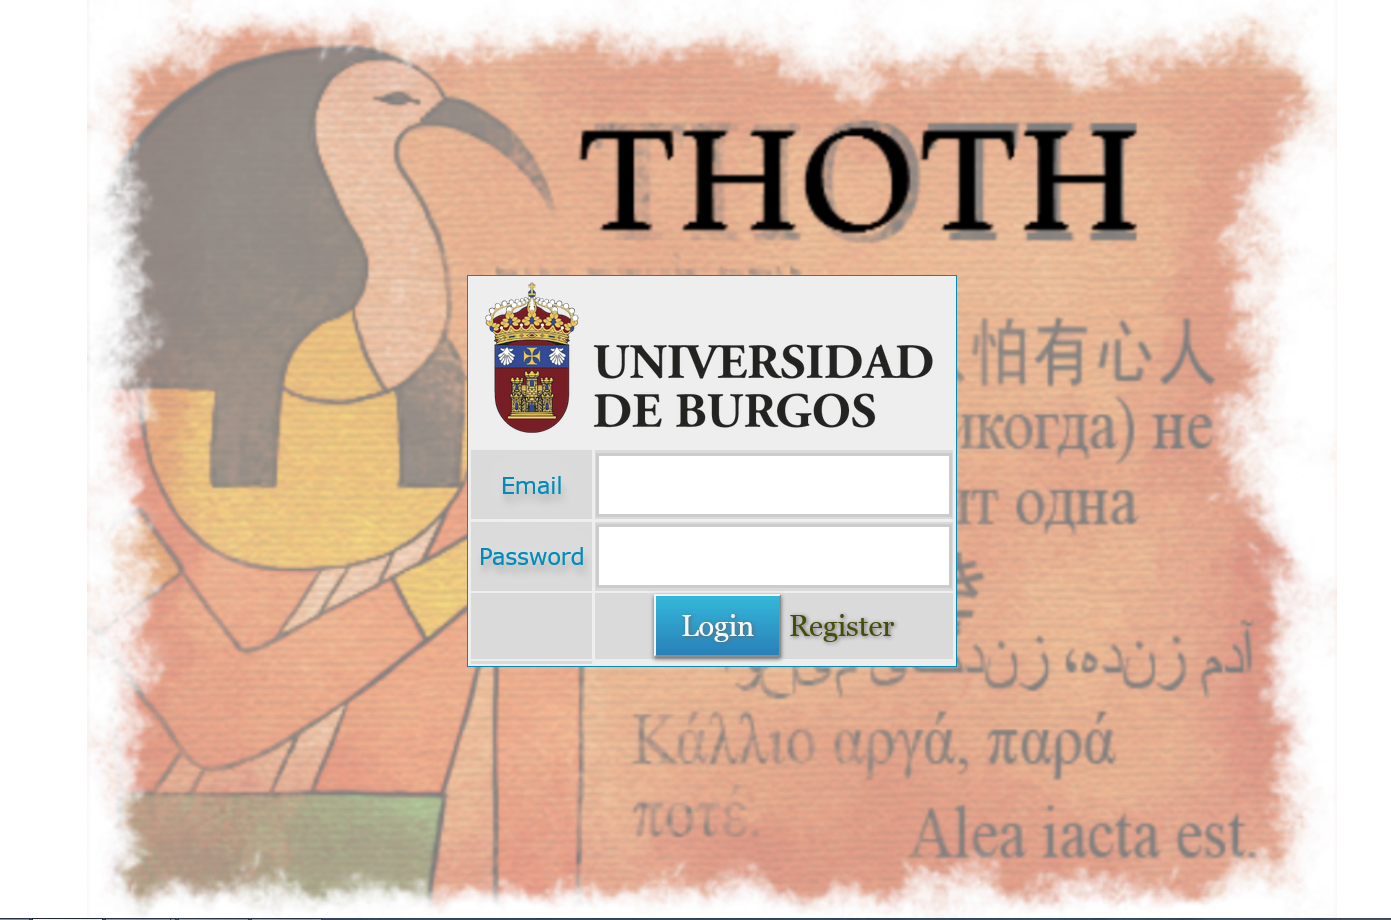
\includegraphics[width=0.50\textwidth]{Login}
\caption{Login en Thoth. Es lo que primero se ve al entrar en la aplicación.}
\label{fig:6.1}
\end{figure}

Al ser la primera vez que utilizamos Thoth no tendremos creada una cuenta, así que debemos registrarnos. Si pulsamos en el link \emph{Register} aparecerá una vista con la siguiente pantalla\ref{fig:6.2}, en la que introduciremos los datos para crear una cuenta. Hay que tener en cuenta que los datos deben estar correctamente rellenados o de lo contrario, la aplicación nos mostrará un error del tipo \emph{Wrong fiel}, campo incorrecto. Si el fallo es el correo electrónico, se marcará el campo en rojo\ref{fig:6.3}. En el caso de que el registro haya sido correcto, se mostrara un mensaje indicativo con el siguiente texto \emph{Registration Success}.

\begin{figure}[h]
\centering
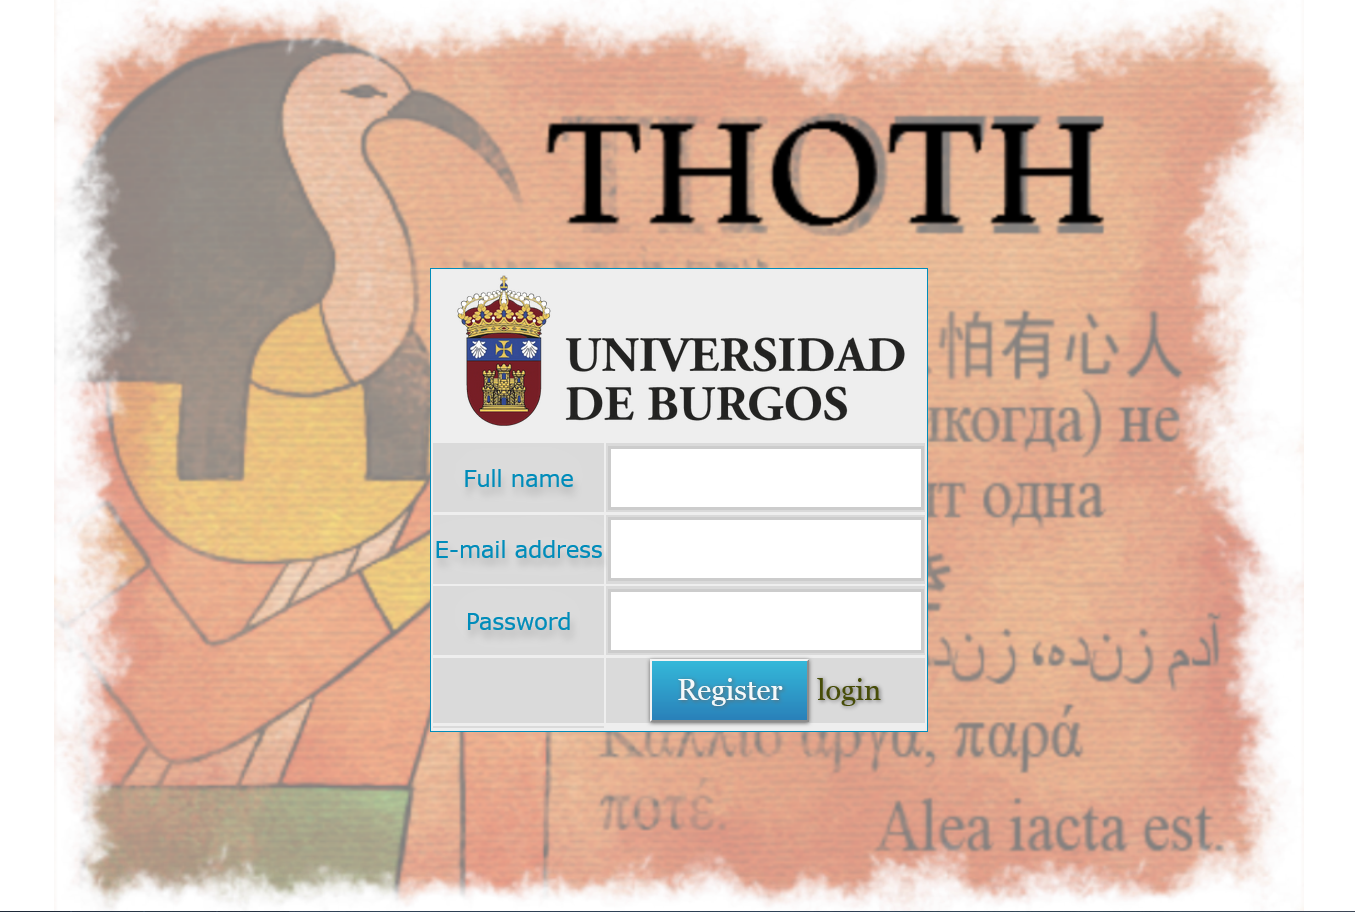
\includegraphics[width=0.50\textwidth]{Registro}
\caption{Pantalla de registro.}
\label{fig:6.2}
\end{figure}

\begin{figure}[h]
\centering
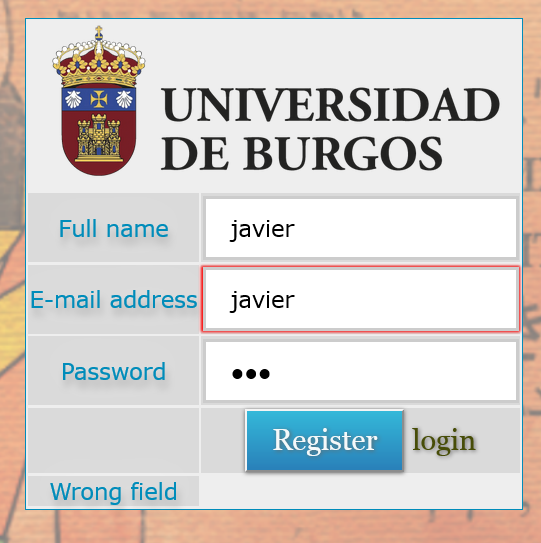
\includegraphics[width=0.40\textwidth]{Email-Error}
\caption{Fallo al introducir el \emph{email}. Se muestra el campo en rojo.}
\label{fig:6.3}
\end{figure}

Una vez registrados, ahora sí, podremos iniciar sesión. Al hacerlo accedemos a la vista principal de la aplicación que consta de tres elementos principales. Un menú, en el que se despliegan diferentes opciones, un panel en el que introducir la gramática y por último una tabla con las características de la gramática. Esta vista se puede apreciar con detalle en la siguiente imagen \ref{fig:6.4}.


\begin{figure}[h]
\centering
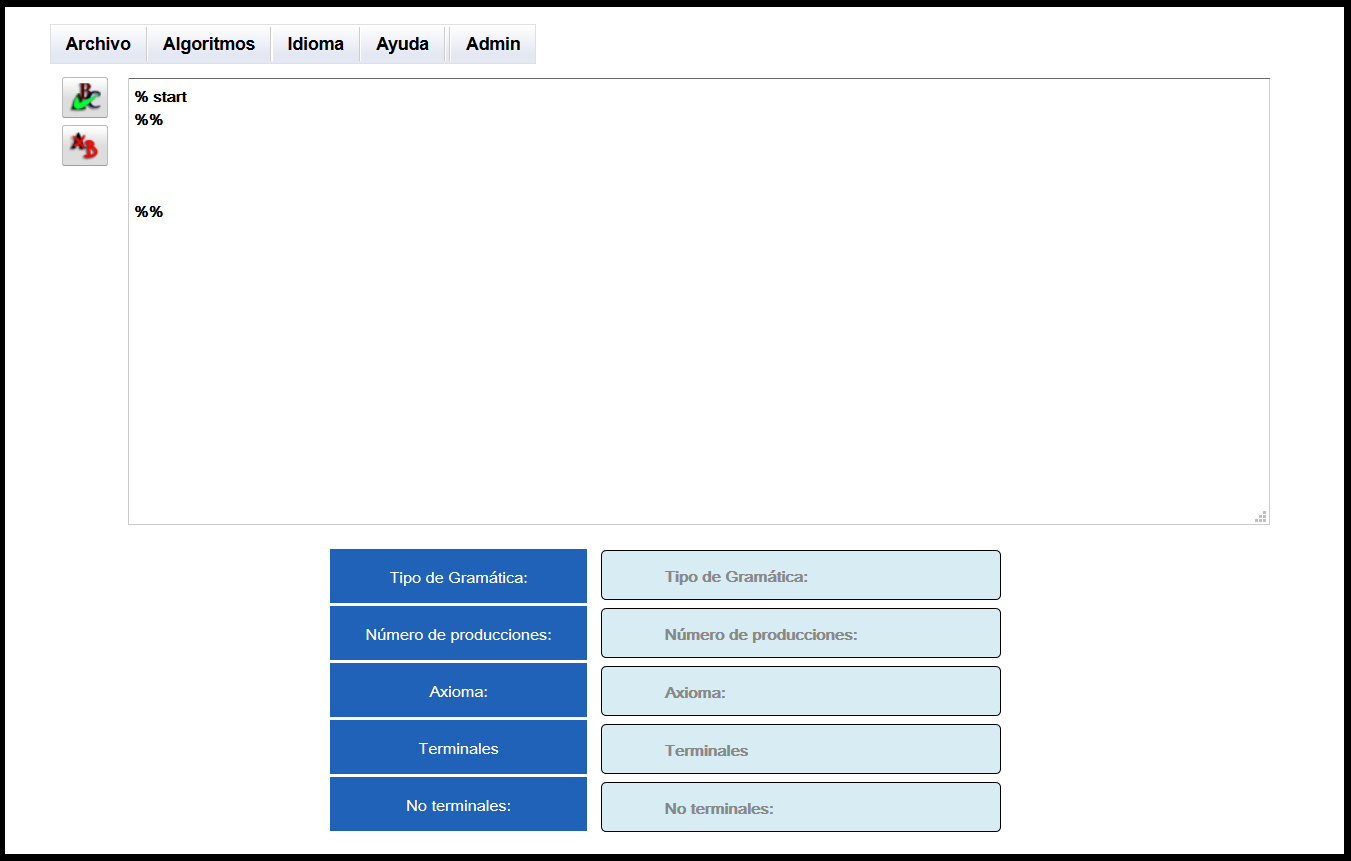
\includegraphics[width=1\textwidth]{Vista-Principal}
\caption{Pantalla principal con el menú de la aplicación y el panel para crear una gramática.}
\label{fig:6.4}
\end{figure}

La parte de azul claro es la que se actualizará, al comprobar una gramática, con las características de esta. Por defecto aparece qué característica es. También podemos apreciar como en el panel aparece ya algo escrito. Esto es para facilitar al usuario la labor al introducir la gramática de escribir ese comienzo. Las gramáticas que se leen en Thoth tienen siempre esa estructura. 

Para empezar, podemos centrarnos en la introducción de la gramática. En el panel podemos copiar, cortar, seleccionar y pegar cualquier carácter. Para comprobar una gramática solo tenemos que pulsar el botón de <<checkear>> en la parte superior. Por otro lado si queremos buscar y reemplazar un símbolo, el botón de renombrado aparece debajo\ref{fig:6.5}. 

\begin{figure}[h]
\centering
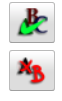
\includegraphics[width=0.1\textwidth]{botones-gramatica}
\caption{En la parte superior comprobar gramática y abajo renombrar. Ambos botones son los mismos que en las otras versiones de Thoth.}
\label{fig:6.5}
\end{figure}

Entonces, comenzamos introduciendo una gramática. En este caso los símbolos $\epsilon$ se representan con la letra E mayúscula y el símbolo \^. Comprobamos la gramática y en la parte inferior aparecen las características de esta \ref{fig:6.6}.  

\begin{figure}[h]
\centering
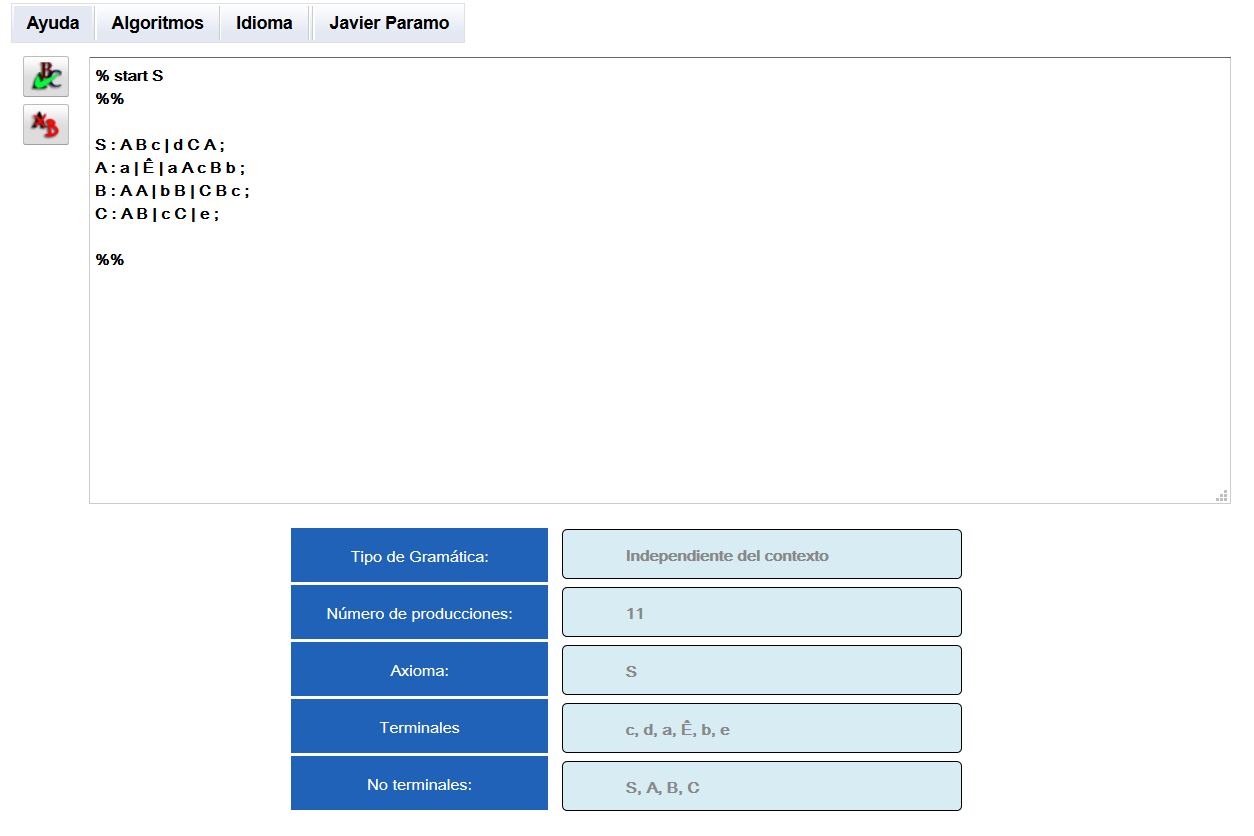
\includegraphics[width=1\textwidth]{comprobando-gramatica}
\caption{Comprobación de una gramática y como se actualiza la tabla inferior.}
\label{fig:6.6}
\end{figure}

Para renombrar aparecerá una ventana con esta forma\ref{fig:6.7}. En la parte superior introducimos el carácter a sustituir. Como se ve, aparece en forma de desplegable los caracteres iguale o similares. En la gramática es diferente la <<a>> que la <<A>>. Abajo se introduce el carácter que le sustituye.

\begin{figure}[h]
\centering
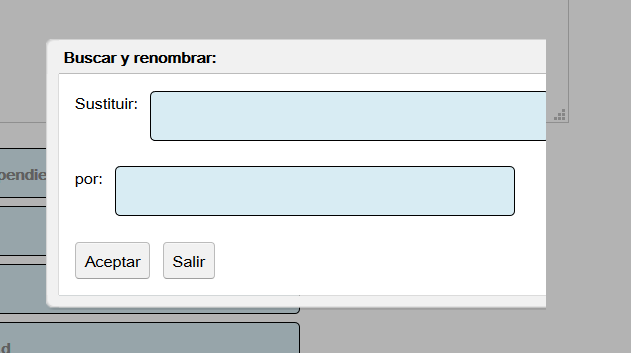
\includegraphics[width=0.40\textwidth]{Renombrado}
\caption{Renombrado de símbolos.}
\label{fig:6.7}
\end{figure}

Cuando se pulsa en aceptar se actualizará la gramática con la sustitución hecha. Entonces habrá que salir del panel.

Dentro de las opciones del menú, quizá la más utilizada es la de elegir uno de los algoritmos a aplicar a la gramática. En el desplegable se pueden ver todas las opciones que hay. Para no extendernos, mostraré las vistas de los algoritmos que sean diferentes a las demás. Antes de aplicar el algoritmo se debe comprobar la gramática, de lo contrario, la aplicación la comprobará automáticamente.

El algoritmo escogido es el de Eliminación de Símbolos Anulables como se puede apreciar en la imagen\ref{fig:6.8}. Es muy similar a los dos primeros algoritmos. Se puede apreciar como se resaltan las producciones en color verde y otras en rojo. Esto sólo ocurre cuando se aplica el algoritmo paso a paso. De lo contrario, no mostrará el proceso, y simplemente aparecerá a un lado la gramática antigua y al otro la nueva.

\begin{figure}[h]
\centering
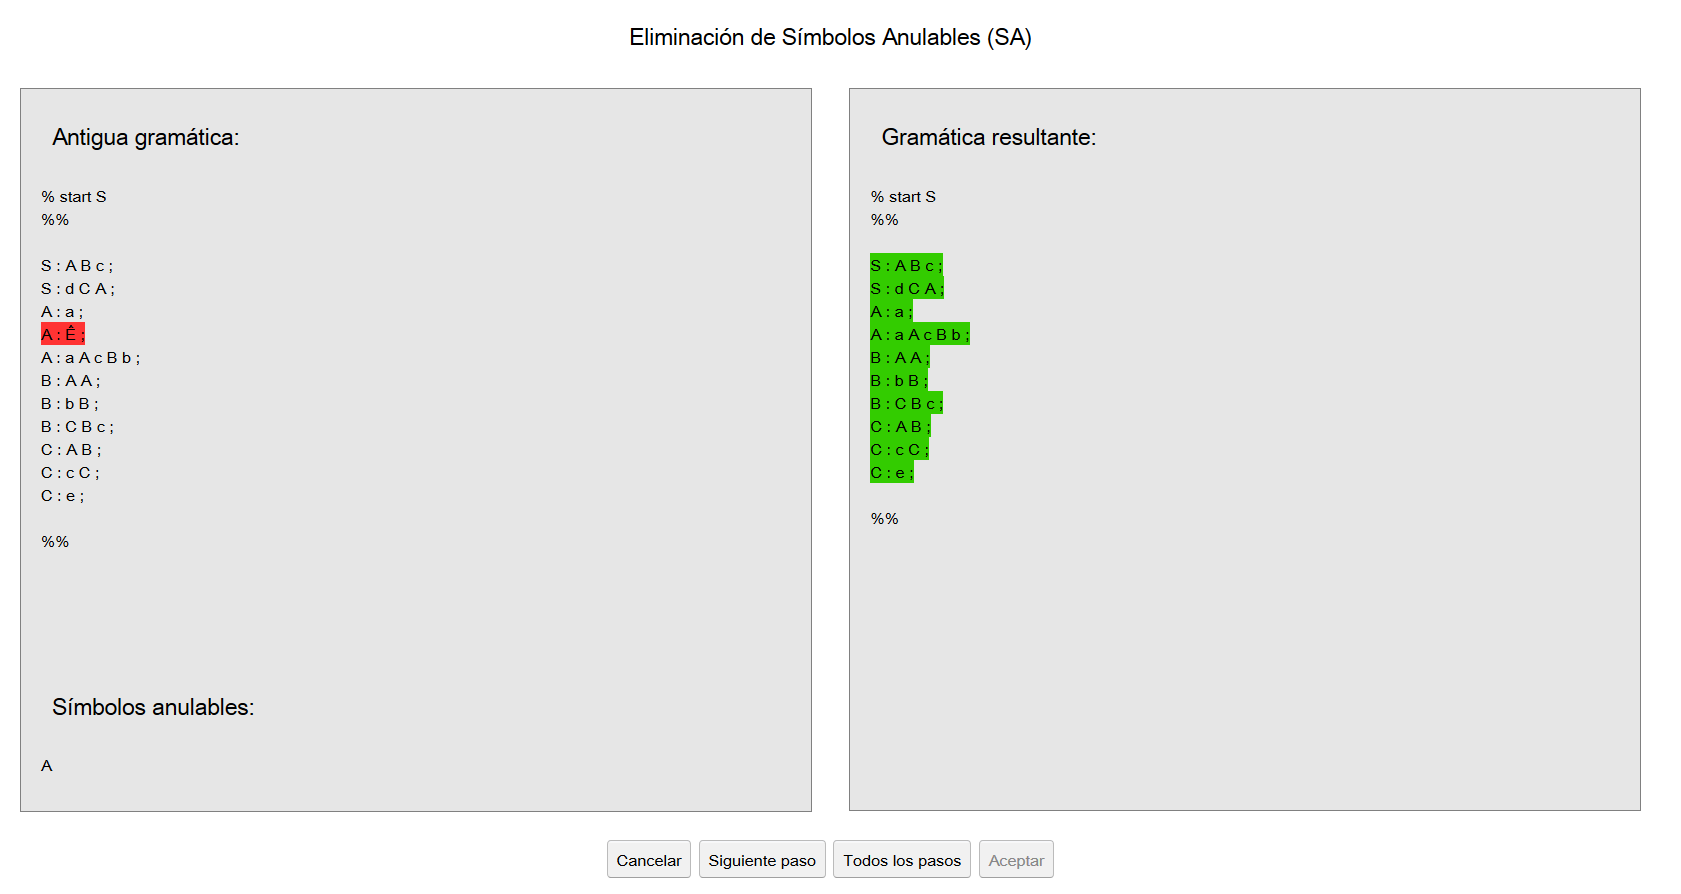
\includegraphics[width=1\textwidth]{vista-algoritmos}
\caption{Ejemplo de una vista del algoritmo Eliminación de SA.}
\label{fig:6.8}
\end{figure}

En verde se iluminan las producciones que pasan a la nueva gramática en ese paso, y en rojo se resalta el símbolo anulable que se está analizando. Si pulsamos en <<cancelar>> se vuelve a la vista principal de edición de gramática con la gramática antigua. Por el contrario se pulsamos en <<aceptar>> volveremos a la vista principal pero con la gramática resultante. El botón aceptar solo se activará una vez se haya terminado de aplicar el algoritmo, de lo contrario no tendría sentido. 

Los demás algoritmos tiene un \emph{modus operandi} parecido, por lo que omitiré el proceso. Resaltar que tanto el algoritmo de Limpieza de Gramática como el de Eliminar Recursividad se aplican de forma directa. Es decir cuando se ejecutan no se pasa a una vista nueva, sino que se actualiza la gramática ya en el panel.

Los algoritmos que cambian bastante en la forma de proceder son l cálculo del First y el Follow y el reconocimiento por medio de TASP. El cálculo de First Follow deriva al reconocimiento con TASP, ya que ambos son algoritmos de análisis ascendente. En el ejemplo de First-Follow con cada botón se crea la tabla correspondiente\ref{fig:6.9}. Los botones de desactivan a mediada que se utilizan.

\begin{figure}[h]
\centering
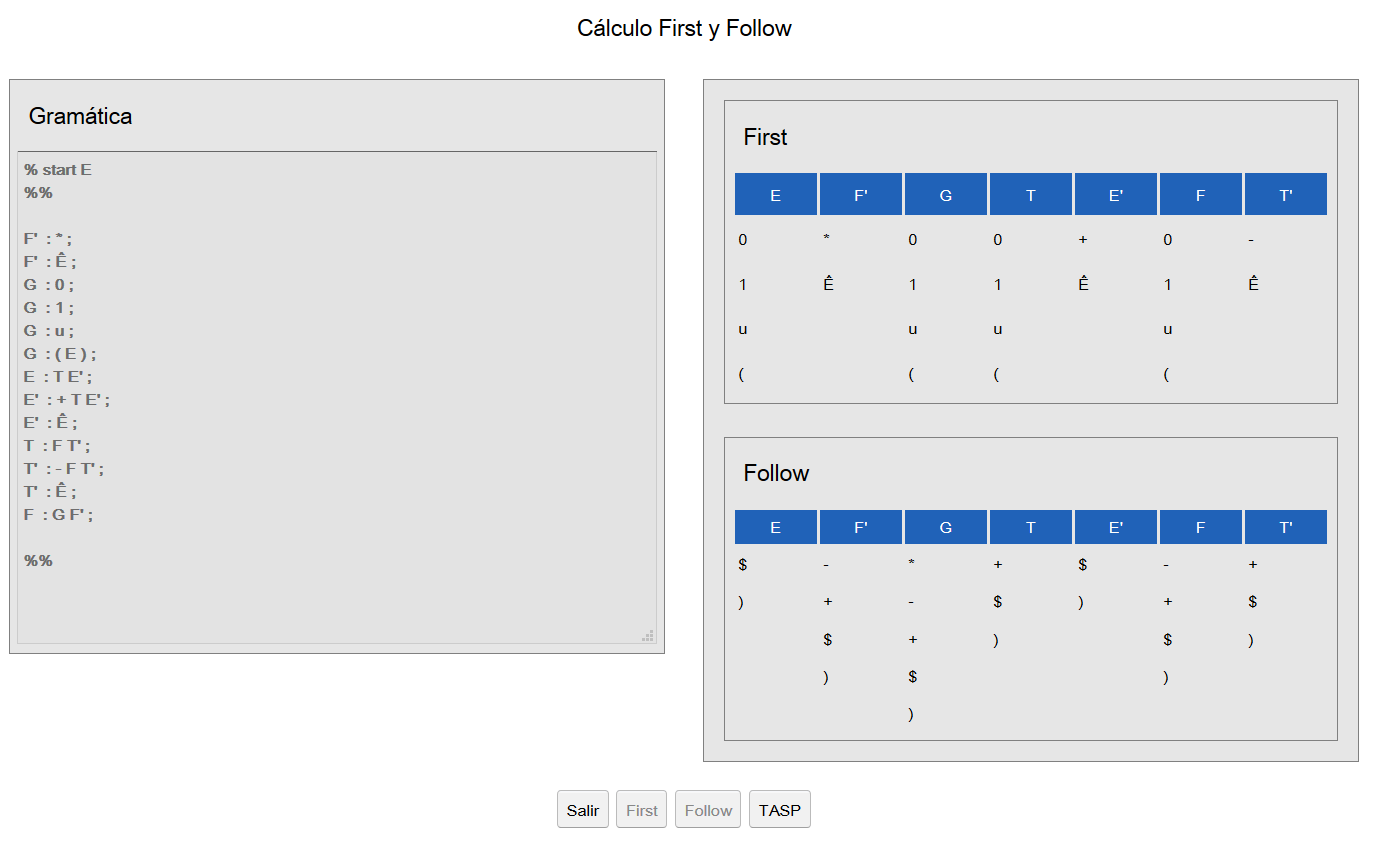
\includegraphics[width=1\textwidth]{calculo-ff}
\caption{Vista del algoritmo para el Cálculo de Fisrt Follow.}
\label{fig:6.9}
\end{figure}

Antes de ejecutar ambos algoritmos se pide confirmación adicional al usuario antes de proceder. Se conservan la forma de las anteriores versiones de Thoth. Como estos dos algoritmos no generan gramática nuevas no existe un botón de aceptar.

Para el reconocimiento con TASP, se muestra primero la Tabla de Análisis Sintáctico Predictivo (TASP) y aparece un recuadro en el que introducir la palabra a analizar\ref{fig:6.10}. Verificamos que es la palabra que queremos, o podemos borrarla con con los dos botones que aparecen a su lado. A continuación se crea la traza. podemos ejecutarla paso a paso o todos los pasos a la vez, el resultado es el mismo. Al terminar de calcular la traza se mostrará un mensaje advirtiendo si se ha reconocido o no la palabra. podremos volver a la vista principal.

\begin{figure}[h]
\centering
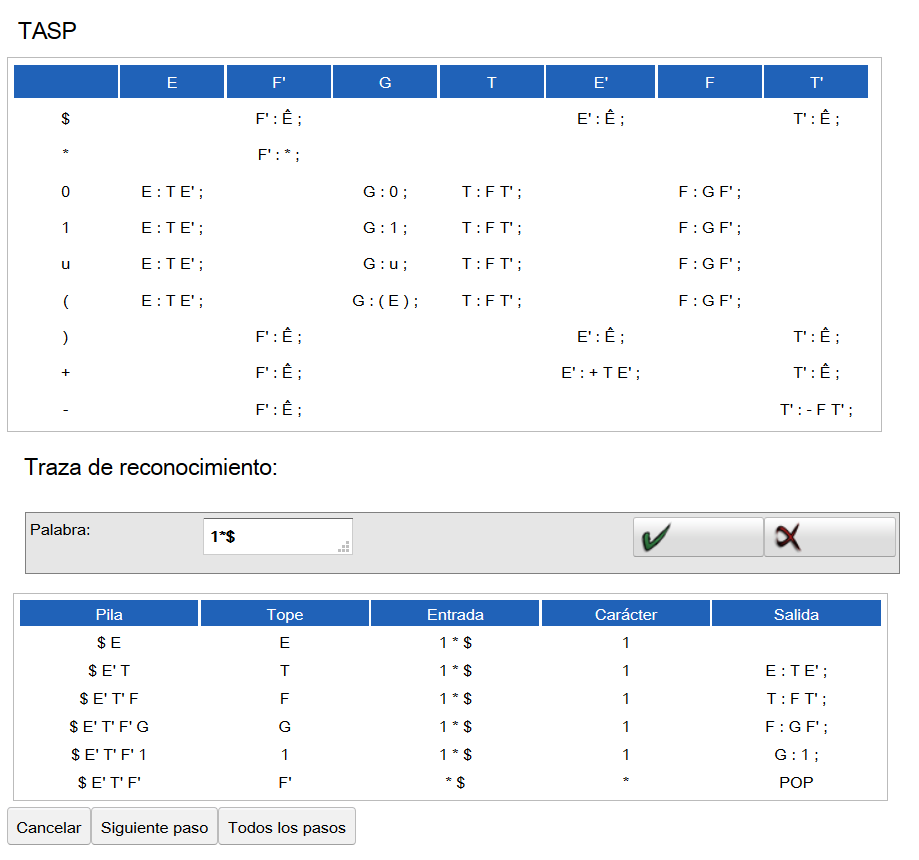
\includegraphics[width=1\textwidth]{reconocimiento-Tasp}
\caption{Vista del reconocimiento con TASP. Se aprecia la zona donde introducir la palabra y los botones.}
\label{fig:6.10}
\end{figure}

Volviendo al menú podemos apreciar que en las opciones aparece el nombre con el que se ha registrado el usuario. Si pulsamos en ello podremos ver como se despliega la opción para cerrar la sesión \ref{fig:6.11}. Al cerrar sesión se volverá a la vista de \emph{login} y deberemos acceder de nuevo escribiendo el correo y la contraseña.

\begin{figure}[h]
\centering
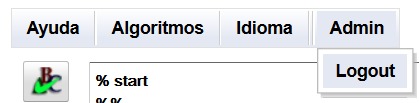
\includegraphics[width=0.40\textwidth]{menu-usuario}
\caption{Menú con el nombre del usuario. El desplegable muestra el cierre de la sesión.}
\label{fig:6.11}
\end{figure}

Siguiendo con el menú, la opción del idioma permite cambiar los textos de la aplicación, al idioma elegido \ref{fig:6.12}. Como la vista se va a reiniciar y la gramática desaparecerá, es necesario mostrar un mensaje que solicita confirmación adicional. Si pulsamos en <<si>> se llevará a cabo el reinicio, y como ya mantenemos una sesión activa, no sera necesario volver a iniciar sesión. Su pulsamos <<no>> el \emph{popup} desaparecerá.

\begin{figure}[h]
\centering
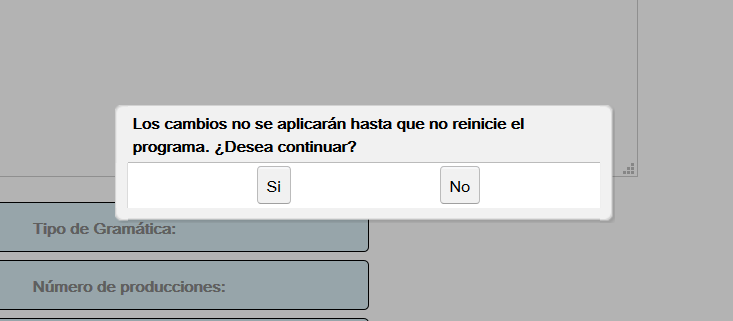
\includegraphics[width=0.40\textwidth]{opcion-idioma}
\caption{Mensaje de confirmación para cambiar el idioma.}
\label{fig:6.12}
\end{figure}

